\documentclass[11pt]{article}
\usepackage[notes]{la}
\lamodule{3}{3}{Cramer's Rule, Volume, and Linear Transformations}
\laxdoc{2.2}
\laxdoc{2.3}
\laxdoc{3.1}
\laxdoc{3.2}

\begin{document}

\section{Cramer's Rule, Volume, and Linear Transformations}

\begin{guide}
In Section 2.2 the equation $A\bv{x}=\bv{b}$ was solved by $\bv{x}=A^{-1}\bv{b}$, and the inverse itself was found by row reducing $[A\ \ I]$. Determinants promise something different: a \emph{formula}, in which every unknown is a ratio of two determinants. Does such a formula exist for $3\times3$ systems, what does it cost, and when is it worth having? The same idea should write down the inverse with cofactors alone. And once $|\det A|$ is known to be the factor by which $A$ multiplies the area of a square (Pause and think~\ref{3.2-think:area}), does it multiply the area of \emph{every} region, a disk for instance?
\end{guide}

\textbf{By the end of this section you should be able to:}
\begin{itemize}
  \item write down the matrix $A_i(\bv{b})$ for each unknown and solve a system by Cramer's Rule, and say when the rule applies;
  \item prove Cramer's Rule from the identity $A\,I_i(\bv{x})=A_i(\bv{b})$ and the product rule, and explain why the hypothesis $\det A\neq0$ is needed;
  \item count the determinants that Cramer's Rule requires, and explain why it is a poor way to solve a large system;
  \item form the adjugate $\operatorname{adj}A$ (the \emph{transpose} of the cofactor matrix) and use $A^{-1}=\frac1{\det A}\operatorname{adj}A$;
  \item compute the area of a parallelogram or a triangle and the volume of a parallelepiped with a determinant, and explain why this works by column operations;
  \item find the area or volume of the image of a region under $\bv{x}\mapsto A\bv{x}$, and explain why the factor is $|\det A|$ and why factors multiply under composition.
\end{itemize}

% ---------------------------------------------------------------------
\subsection*{Cramer's Rule}

Before the general rule, solve a general $2\times2$ system by elimination and watch the number $ad-bc$ appear:
\begin{align*}
a_{11}x_1+a_{12}x_2&=b_1,\\
a_{21}x_1+a_{22}x_2&=b_2.
\end{align*}
Multiply the first equation by $a_{22}$ and the second by $a_{12}$ and subtract; the unknown $x_2$ disappears:
\[
(a_{11}a_{22}-a_{12}a_{21})\,x_1=b_1a_{22}-a_{12}b_2 .
\]
Multiply the first equation by $a_{21}$ and the second by $a_{11}$ and subtract; now $x_1$ disappears:
\[
(a_{11}a_{22}-a_{12}a_{21})\,x_2=a_{11}b_2-a_{21}b_1 .
\]
Both coefficients are $\det A$ for the coefficient matrix $A$. If $\det A\neq0$ we can divide, and both numerators are determinants too:
\[
x_1=\frac{\begin{vmatrix}b_1&a_{12}\\b_2&a_{22}\end{vmatrix}}{\begin{vmatrix}a_{11}&a_{12}\\a_{21}&a_{22}\end{vmatrix}},\qquad
x_2=\frac{\begin{vmatrix}a_{11}&b_1\\a_{21}&b_2\end{vmatrix}}{\begin{vmatrix}a_{11}&a_{12}\\a_{21}&a_{22}\end{vmatrix}}.
\]
The numerator of $x_1$ is the determinant of $A$ with its \emph{first column replaced by the right-hand side}; the numerator of $x_2$ replaces the second column. This is the pattern that the questions at the end of Section 3.2 asked about. Does it persist for $n$ unknowns? We need a name for the matrices involved.

\begin{defn}{Column replacement}{replace}
Let $A=[\bv{a}_1\ \cdots\ \bv{a}_n]$ be an $n\times n$ matrix and let $\bv{b}$ be a vector in $\R^n$. For $i=1,\dots,n$ let $A_i(\bv{b})$ be the matrix obtained from $A$ by replacing column $i$ by $\bv{b}$:
\[
A_i(\bv{b})=[\bv{a}_1\ \cdots\ \bv{a}_{i-1}\ \ \bv{b}\ \ \bv{a}_{i+1}\ \cdots\ \bv{a}_n].
\]
In the same way, for $\bv{x}$ in $\R^n$ let $I_i(\bv{x})$ be the identity matrix with column $i$ replaced by $\bv{x}$:
\[
I_i(\bv{x})=[\bv{e}_1\ \cdots\ \bv{e}_{i-1}\ \ \bv{x}\ \ \bv{e}_{i+1}\ \cdots\ \bv{e}_n].
\]
\end{defn}

Do not confuse $A_i(\bv{b})$, which has one subscript and an argument, with the submatrix $A_{ij}$ of Section 3.1, which has two subscripts and \emph{deletes} a row and a column.

\begin{thm}{Cramer's Rule}{cramer}
Let $A$ be an invertible $n\times n$ matrix. For every $\bv{b}$ in $\R^n$, the unique solution $\bv{x}$ of $A\bv{x}=\bv{b}$ has the entries
\[
x_i=\frac{\det A_i(\bv{b})}{\det A},\qquad i=1,2,\dots,n.
\]
\end{thm}

\begin{proof}
By Theorem~\ref{2.2-thm:solve} the equation has exactly one solution $\bv{x}$, and $\det A\neq0$ by Theorem~\ref{3.2-thm:invertible}. Fix $i$ and multiply $A$ by $I_i(\bv{x})$ one column at a time (Section 2.1). For $j\neq i$ the $j$th column of the product is $A\bv{e}_j=\bv{a}_j$, and the $i$th column is $A\bv{x}=\bv{b}$. Therefore
\begin{equation}\label{eq:key}
A\,I_i(\bv{x})=[\bv{a}_1\ \cdots\ \bv{b}\ \cdots\ \bv{a}_n]=A_i(\bv{b}).
\end{equation}
Take determinants and use the product rule (Theorem~\ref{3.2-thm:product}):
\[
(\det A)\,\bigl(\det I_i(\bv{x})\bigr)=\det A_i(\bv{b}).
\]
Row $i$ of $I_i(\bv{x})$ is $(0,\dots,0,x_i,0,\dots,0)$, because the $i$th entry of every $\bv{e}_j$ with $j\neq i$ is $0$. Expand along row $i$ (Theorem~\ref{3.1-thm:expansion}): the only term is $x_i$, in position $(i,i)$ with sign $+$, times the determinant of the matrix that remains after deleting row $i$ and column $i$, which is $I_{n-1}$. Hence $\det I_i(\bv{x})=x_i$ and $(\det A)\,x_i=\det A_i(\bv{b})$. Divide by $\det A\neq0$.
\end{proof}

\begin{think}{Why does the formula work?}{why}
(a)~For $A=\begin{bmatrix}a&b\\c&d\end{bmatrix}$ and $\bv{x}=(x_1,x_2)$ write out $I_1(\bv{x})$ and $I_2(\bv{x})$ and multiply each by $A$ to confirm \eqref{eq:key}, with $\bv{b}=A\bv{x}$. (b)~In words: why do the columns of $A\,I_i(\bv{x})$ other than column $i$ agree with those of $A$, and why is column $i$ equal to $\bv{b}$? (c)~Write $I_3(\bv{x})$ for $n=3$. What kind of matrix is it, and why is its determinant $x_3$ without any expansion? Is $I_2(\bv{x})$ of the same kind?
\end{think}

\begin{exmp}{Cramer's Rule for a $2\times2$ system}{twoby}
Solve $2x_1+5x_2=1$, \ $3x_1+7x_2=2$. Here $A=\begin{bmatrix}2&5\\3&7\end{bmatrix}$, $\bv{b}=(1,2)$ and $\det A=14-15=-1\neq0$. Replace column $1$ and then column $2$ of $A$ by $\bv{b}$:
\[
A_1(\bv{b})=\begin{bmatrix}1&5\\2&7\end{bmatrix},\qquad A_2(\bv{b})=\begin{bmatrix}2&1\\3&2\end{bmatrix}.
\]
Then
\[
x_1=\frac{\det A_1(\bv{b})}{\det A}=\frac{7-10}{-1}=3,\qquad x_2=\frac{\det A_2(\bv{b})}{\det A}=\frac{4-3}{-1}=-1.
\]
Check: $2\cdot3+5(-1)=1$ and $3\cdot3+7(-1)=2$.
\end{exmp}

\begin{exmp}{Cramer's Rule for a $3\times3$ system}{threeby}
Solve $x_1+2x_3=7$, \ $2x_1+x_2-x_3=-3$, \ $3x_2+x_3=-3$. The coefficient matrix and right-hand side are
\[
A=\begin{bmatrix}1&0&2\\2&1&-1\\0&3&1\end{bmatrix},\qquad\bv{b}=\begin{bmatrix}7\\-3\\-3\end{bmatrix}.
\]
Expanding down column $1$: $\det A=1\begin{vmatrix}1&-1\\3&1\end{vmatrix}-2\begin{vmatrix}0&2\\3&1\end{vmatrix}=1(4)-2(-6)=16$. Since $\det A\neq0$, Cramer's Rule applies. Each numerator is the determinant of $A$ with one column replaced by $\bv{b}$:
\begin{align*}
\det A_1(\bv{b})&=\begin{vmatrix}7&0&2\\-3&1&-1\\-3&3&1\end{vmatrix}=7\begin{vmatrix}1&-1\\3&1\end{vmatrix}+2\begin{vmatrix}-3&1\\-3&3\end{vmatrix}=7(4)+2(-6)=16,\\
\det A_2(\bv{b})&=\begin{vmatrix}1&7&2\\2&-3&-1\\0&-3&1\end{vmatrix}=1\begin{vmatrix}-3&-1\\-3&1\end{vmatrix}-2\begin{vmatrix}7&2\\-3&1\end{vmatrix}=1(-6)-2(13)=-32,\\
\det A_3(\bv{b})&=\begin{vmatrix}1&0&7\\2&1&-3\\0&3&-3\end{vmatrix}=1\begin{vmatrix}1&-3\\3&-3\end{vmatrix}-2\begin{vmatrix}0&7\\3&-3\end{vmatrix}=1(6)-2(-21)=48.
\end{align*}
So $x_1=\frac{16}{16}=1$, \ $x_2=\frac{-32}{16}=-2$, \ $x_3=\frac{48}{16}=3$. Check in the first equation: $1+2\cdot3=7$; in the second: $2-2-3=-3$; in the third: $-6+3=-3$.
\end{exmp}

\begin{kc}{Which column?}{replace}
Let $A=\begin{bmatrix}1&4&7\\2&5&8\\3&6&10\end{bmatrix}$ (the matrix of Example~\ref{3.2-ex:indep}, with $\det A=-3$) and $\bv{b}=(1,0,2)$. (a)~Write down the matrices $A_2(\bv{b})$ and $A_3(\bv{b})$. (b)~What is the denominator of each of $x_1,x_2,x_3$? (c)~Compute $x_1$ by Cramer's Rule.
\end{kc}

\begin{warn}[Column trap]
Cramer's Rule has two easy slips. (i)~\emph{The wrong column.} The numerator of $x_i$ is built by replacing column $i$, the column that multiplies $x_i$. A student who wants $x_1$ in Example~\ref{ex:twoby} but puts $\bv{b}$ into column $2$ computes $\det\begin{bmatrix}2&1\\3&2\end{bmatrix}/(-1)=-1$ and reports $x_1=-1$; that number is $x_2$, while $x_1=3$. (ii)~\emph{Building $A_i(\bv{b})$ from the wrong matrix.} Every $A_i(\bv{b})$ is built from the original $A$. If you replace column $2$ of the already modified matrix $A_1(\bv{b})=\begin{bmatrix}1&5\\2&7\end{bmatrix}$ you get $\begin{bmatrix}1&1\\2&2\end{bmatrix}$, whose determinant is $0$, and you would report $x_2=0$ instead of $-1$. And the denominator is always $\det A$, the same for every unknown; it is never $\det A_i(\bv{b})$.
\end{warn}

\begin{exmp}{A parameter}{param}
For which values of $h$ does Cramer's Rule apply to the system $hx_1+2x_2=1$, \ $8x_1+hx_2=2$, and what is the solution then? The coefficient matrix is $A(h)=\begin{bmatrix}h&2\\8&h\end{bmatrix}$ and $\det A(h)=h^2-16=(h-4)(h+4)$, so the rule applies exactly when $h\neq4$ and $h\neq-4$. For those $h$, with $\bv{b}=(1,2)$,
\[
\det A_1(\bv{b})=\begin{vmatrix}1&2\\2&h\end{vmatrix}=h-4,\qquad\det A_2(\bv{b})=\begin{vmatrix}h&1\\8&2\end{vmatrix}=2h-8=2(h-4),
\]
and therefore
\[
x_1=\frac{h-4}{(h-4)(h+4)}=\frac1{h+4},\qquad x_2=\frac{2(h-4)}{(h-4)(h+4)}=\frac2{h+4}.
\]
Check with $h=0$: the system is $2x_2=1$, $8x_1=2$, with solution $(\tfrac14,\tfrac12)$, and the formulas give $\tfrac14$ and $\tfrac24$. The two excluded values behave differently, and the rule says nothing about them. For $h=4$ the second equation $8x_1+4x_2=2$ is twice the first, $4x_1+2x_2=1$, so there are infinitely many solutions. For $h=-4$ twice the first equation is $-8x_1+4x_2=2$, and adding it to the second gives $0=4$: there is no solution.
\end{exmp}

\begin{think}{Why do we need $\det A\neq0$?}{hyp}
(a)~Which step in the proof of Theorem~\ref{thm:cramer} fails if $\det A=0$? (b)~Let $A=\begin{bmatrix}1&2\\2&4\end{bmatrix}$. Compute $\det A_1(\bv{b})$ and $\det A_2(\bv{b})$ for $\bv{b}=(3,6)$ and for $\bv{b}=(3,5)$. Which of the two systems has solutions? (c)~If $\det A=0$ and $A\bv{x}=\bv{b}$ has a solution, the proof still gives $(\det A)\,x_i=\det A_i(\bv{b})$. What does this force on every $\det A_i(\bv{b})$? What can you conclude when some $\det A_i(\bv{b})$ is not $0$, and what can you not conclude when all of them are $0$?
\end{think}

\begin{exmp}{When $\det A=0$}{singular}
Let $A=\begin{bmatrix}1&2&3\\4&5&6\\7&8&9\end{bmatrix}$, whose determinant is $0$ (Example~\ref{3.2-ex:zerorow}). Cramer's Rule does not apply. Look at what the numerators say.

\textbf{(a)}~$\bv{b}=(1,2,3)$. Here
\[
\det A_1(\bv{b})=\begin{vmatrix}1&2&3\\2&5&6\\3&8&9\end{vmatrix}=0,\quad
\det A_2(\bv{b})=\begin{vmatrix}1&1&3\\4&2&6\\7&3&9\end{vmatrix}=0,\quad
\det A_3(\bv{b})=\begin{vmatrix}1&2&1\\4&5&2\\7&8&3\end{vmatrix}=0,
\]
and row reduction shows that the system is consistent, with infinitely many solutions:
\begin{align*}
\begin{amat}{ccc|c}1&2&3&1\\4&5&6&2\\7&8&9&3\end{amat}
&\rops{R_2-4R_1,\ R_3-7R_1}
\begin{amat}{ccc|c}1&2&3&1\\0&-3&-6&-2\\0&-6&-12&-4\end{amat}
\rops{R_3-2R_2}
\begin{amat}{ccc|c}1&2&3&1\\0&-3&-6&-2\\0&0&0&0\end{amat}.
\end{align*}
The free variable $x_3=t$ gives $x_2=\tfrac23-2t$ and $x_1=-\tfrac13+t$.

\textbf{(b)}~$\bv{b}=(1,0,0)$. Now $\det A_1(\bv{b})=\begin{vmatrix}1&2&3\\0&5&6\\0&8&9\end{vmatrix}=1(45-48)=-3\neq0$. If a solution existed we would have $0\cdot x_1=-3$, which is impossible, so the system is inconsistent. Row reduction agrees:
\begin{align*}
\begin{amat}{ccc|c}1&2&3&1\\4&5&6&0\\7&8&9&0\end{amat}
&\rops{R_2-4R_1,\ R_3-7R_1}
\begin{amat}{ccc|c}1&2&3&1\\0&-3&-6&-4\\0&-6&-12&-7\end{amat}
\rops{R_3-2R_2}
\begin{amat}{ccc|c}1&2&3&1\\0&-3&-6&-4\\0&0&0&1\end{amat}.
\end{align*}
In both cases all three numerators have the same pattern as in the $2\times2$ matrix of Pause and think~\ref{think:hyp}: a nonzero numerator proves that there is no solution, while all numerators equal to $0$ proves nothing.
\end{exmp}

\begin{think}{Is Cramer's Rule a good method?}{cost}
For an $n\times n$ system, Cramer's Rule needs $\det A$ and the $n$ determinants $\det A_i(\bv{b})$. (a)~How many $n\times n$ determinants is that? (b)~If each is computed by cofactor expansion, which uses more than $n!$ multiplications (Example~\ref{3.1-ex:cost}), how many multiplications does the rule need for $n=10$? (c)~Suppose each determinant is computed by row reduction, at about $\tfrac23n^3$ operations (Pause and think~\ref{3.2-think:cost}). Estimate the total for $n=100$, and compare it with row reducing $[A\ \ \bv{b}]$ once, which solves the system with about $\tfrac23n^3$ operations. (d)~By what factor is Cramer's Rule slower? (e)~Give two reasons why the rule is still worth knowing.
\end{think}

% ---------------------------------------------------------------------
\subsection*{A formula for the inverse}

The columns of $A^{-1}$ are the solutions of $A\bv{x}=\bv{e}_j$ (Pause and think~\ref{2.2-think:colsinv} and Example~\ref{2.2-ex:onecol}). Cramer's Rule can therefore write down every entry of the inverse. The result is stated with cofactors, so we recall them: the $(i,j)$-cofactor of $A$ is $C_{ij}=(-1)^{i+j}\det A_{ij}$ (Definition~\ref{3.1-def:cofactor}).

\begin{defn}{The adjugate}{adjugate}
Let $A$ be an $n\times n$ matrix with $n\geq2$. The \emph{cofactor matrix} of $A$ is $C=[C_{ij}]$. The \emph{adjugate} (or \emph{classical adjoint}) of $A$ is the \textbf{transpose} of the cofactor matrix:
\[
\operatorname{adj}A=C\T=\begin{bmatrix}C_{11}&C_{21}&\cdots&C_{n1}\\C_{12}&C_{22}&\cdots&C_{n2}\\\vdots&\vdots&&\vdots\\C_{1n}&C_{2n}&\cdots&C_{nn}\end{bmatrix}.
\]
The $(i,j)$-entry of $\operatorname{adj}A$ is the cofactor $C_{ji}$.
\end{defn}

\begin{thm}{The adjugate formula for the inverse}{inverse}
If $A$ is an invertible $n\times n$ matrix, then
\[
A^{-1}=\frac1{\det A}\operatorname{adj}A .
\]
\end{thm}

\begin{proof}
The $j$th column of $A^{-1}$ is the solution of $A\bv{x}=\bv{e}_j$. By Cramer's Rule its $i$th entry, which is the $(i,j)$-entry of $A^{-1}$, is
\[
(A^{-1})_{ij}=\frac{\det A_i(\bv{e}_j)}{\det A}.
\]
The matrix $A_i(\bv{e}_j)$ has column $i$ equal to $\bv{e}_j$, whose only nonzero entry is a $1$ in row $j$. Expand along that column (Theorem~\ref{3.1-thm:expansion}). Deleting row $j$ and column $i$ of $A_i(\bv{e}_j)$ leaves the submatrix $A_{ji}$ of $A$, because the other columns were not changed, so
\[
\det A_i(\bv{e}_j)=(-1)^{j+i}\det A_{ji}=C_{ji}.
\]
Hence $(A^{-1})_{ij}=C_{ji}/\det A$, which is the $(i,j)$-entry of $\frac1{\det A}\operatorname{adj}A$.
\end{proof}

\textbf{Check with the $2\times2$ formula.} For $A=\begin{bmatrix}a&b\\c&d\end{bmatrix}$ the cofactors are $C_{11}=d$, $C_{12}=-c$, $C_{21}=-b$ and $C_{22}=a$. The cofactor matrix is $\begin{bmatrix}d&-c\\-b&a\end{bmatrix}$ and its transpose is $\operatorname{adj}A=\begin{bmatrix}d&-b\\-c&a\end{bmatrix}$. The theorem says $A^{-1}=\frac1{ad-bc}\begin{bmatrix}d&-b\\-c&a\end{bmatrix}$, which is Theorem~\ref{2.2-thm:twobytwo}. The transpose is what moves $-c$ (the cofactor of $b$) into the position that $c$ occupied in $A$.

\begin{exmp}{An adjugate and an inverse for a $3\times3$ matrix}{adjthree}
Let $A=\begin{bmatrix}2&0&1\\3&1&0\\1&2&2\end{bmatrix}$. The nine cofactors are
\begin{align*}
C_{11}&=+\begin{vmatrix}1&0\\2&2\end{vmatrix}=2, & C_{12}&=-\begin{vmatrix}3&0\\1&2\end{vmatrix}=-6, & C_{13}&=+\begin{vmatrix}3&1\\1&2\end{vmatrix}=5,\\
C_{21}&=-\begin{vmatrix}0&1\\2&2\end{vmatrix}=2, & C_{22}&=+\begin{vmatrix}2&1\\1&2\end{vmatrix}=3, & C_{23}&=-\begin{vmatrix}2&0\\1&2\end{vmatrix}=-4,\\
C_{31}&=+\begin{vmatrix}0&1\\1&0\end{vmatrix}=-1, & C_{32}&=-\begin{vmatrix}2&1\\3&0\end{vmatrix}=3, & C_{33}&=+\begin{vmatrix}2&0\\3&1\end{vmatrix}=2.
\end{align*}
Expanding along row $1$, $\det A=2\cdot2+0\cdot(-6)+1\cdot5=9$. The cofactor matrix and its transpose are
\[
C=\begin{bmatrix}2&-6&5\\2&3&-4\\-1&3&2\end{bmatrix},\qquad
\operatorname{adj}A=C\T=\begin{bmatrix}2&2&-1\\-6&3&3\\5&-4&2\end{bmatrix},
\]
so $A^{-1}=\tfrac19\operatorname{adj}A$. Check that $A\operatorname{adj}A=(\det A)I$:
\[
\begin{bmatrix}2&0&1\\3&1&0\\1&2&2\end{bmatrix}\begin{bmatrix}2&2&-1\\-6&3&3\\5&-4&2\end{bmatrix}=\begin{bmatrix}9&0&0\\0&9&0\\0&0&9\end{bmatrix}.
\]
If only one entry of the inverse is needed, one cofactor suffices: $(A^{-1})_{32}=C_{23}/\det A=-\tfrac49$. For the whole inverse, however, this computation took nine $2\times2$ determinants and a $3\times3$ determinant, while row reducing $[A\ \ I]$ (Section 2.2) is shorter, and the gap grows quickly with the size. The value of the formula is that it \emph{displays} the inverse. (The identity $A\operatorname{adj}A=(\det A)I$ also holds when $\det A=0$, but we only need the invertible case.)
\end{exmp}

\begin{warn}[Transpose trap]
The adjugate is the \emph{transpose} of the cofactor matrix, not the cofactor matrix itself. In Example~\ref{ex:adjthree} the untransposed matrix $C$ does not give an inverse: the first row of $A$ times the first column of $C$ is $(2,0,1)\cdot(2,2,-1)=3$, not $9$. In a $2\times2$ matrix the only visible effect of the transpose is where $-b$ and $-c$ sit, which is why the slip is easy to make and easy to miss. Always check an adjugate by computing one or two entries of $A\operatorname{adj}A$: they must be $\det A$ on the diagonal and $0$ off it.
\end{warn}

\begin{kc}{Adjugates}{adj}
(a)~Find $\operatorname{adj}A$ and $A^{-1}$ for $A=\begin{bmatrix}3&1\\4&2\end{bmatrix}$. (b)~Find $\operatorname{adj}A$ and $A^{-1}$ for the upper triangular matrix $A=\begin{bmatrix}1&1&0\\0&1&1\\0&0&1\end{bmatrix}$. (c)~A student writes the \emph{cofactor matrix} of the matrix in~(b), which is lower triangular, as $A^{-1}$. Multiply it by $A$ and say what goes wrong.
\end{kc}

% ---------------------------------------------------------------------
\subsection*{Determinants as area and volume}

In Pause and think~\ref{3.2-think:area} we met $|\det A|$ as the factor by which $A$ multiplies areas, and we used the product rule (Theorem~\ref{3.2-thm:product}) to see that this factor multiplies, so it should work for every invertible matrix. Here we prove the underlying fact directly, for the parallelogram spanned by \emph{any} two vectors and the parallelepiped spanned by any three, and then we go beyond squares: what does a matrix do to the area of an arbitrary region? The parallelogram spanned by $\bv{a}_1,\bv{a}_2$ is the set of points $s\bv{a}_1+t\bv{a}_2$ with $0\leq s,t\leq1$; the parallelepiped spanned by $\bv{a}_1,\bv{a}_2,\bv{a}_3$ is the set of $s\bv{a}_1+t\bv{a}_2+u\bv{a}_3$ with $0\leq s,t,u\leq1$. They are the images of the unit square and the unit cube.

\begin{thm}{Determinants as area and volume}{area}
If $A=[\bv{a}_1\ \bv{a}_2]$ is a $2\times2$ matrix, the area of the parallelogram spanned by $\bv{a}_1$ and $\bv{a}_2$ is $|\det A|$. If $A=[\bv{a}_1\ \bv{a}_2\ \bv{a}_3]$ is $3\times3$, the volume of the parallelepiped spanned by $\bv{a}_1,\bv{a}_2,\bv{a}_3$ is $|\det A|$.
\end{thm}

\begin{proof}
We use three facts about area and volume. \textbf{(F1)} \emph{Adding a multiple of one spanning vector to another does not change the area or volume.} In the plane, the parallelogram spanned by $\bv{a}_1$ and $\bv{a}_2+c\bv{a}_1$ has the same base $\bv{a}_1$ and the same height (the distance from the tip of the second vector to the line through $\bv{0}$ and $\bv{a}_1$), because $c\bv{a}_1$ points along that line. In space, adding to $\bv{a}_3$ a combination of $\bv{a}_1$ and $\bv{a}_2$ keeps the base parallelogram and the height above its plane. \textbf{(F2)} \emph{Interchanging two spanning vectors does not change the set.} \textbf{(F3)} A rectangle with sides $|d_1|,|d_2|$ along the axes has area $|d_1d_2|$, and a box with edges $|d_1|,|d_2|,|d_3|$ along the axes has volume $|d_1d_2d_3|$.

By Theorem~\ref{3.2-thm:colops}, a column replacement does not change $\det A$ and an interchange only changes its sign, so neither changes $|\det A|$. By (F1) and (F2) neither changes the area or the volume.

\emph{Case $\det A=0$.} Then $A$ is not invertible (Theorem~\ref{3.2-thm:invertible}), so its columns are linearly dependent (Theorem~\ref{2.3-thm:imt}). In the plane one column is a multiple of the other, and the parallelogram lies on a line; in space one column is a combination of the other two, and the parallelepiped lies in a plane. Area and volume are $0=|\det A|$.

\emph{Case $\det A\neq0$.} Reduce $A$ to a diagonal matrix by column interchanges and replacements. For $A=\begin{bmatrix}a&b\\c&d\end{bmatrix}$: if $a=0$, then $\det A=-bc\neq0$ forces $b\neq0$, and interchanging the columns puts a nonzero entry in position $(1,1)$. With $a\neq0$, the replacement $C_2-\frac baC_1$ makes the $(1,2)$ entry $0$ and leaves a lower triangular matrix $\begin{bmatrix}a&0\\c&e\end{bmatrix}$ with $e=\det A/a\neq0$. The replacement $C_1-\frac ceC_2$ then clears the $c$. The result is $\operatorname{diag}(a,e)$. In three dimensions the recipe is the same: (1)~interchange columns, if necessary, to make $a_{11}\neq0$ (row $1$ is not zero, since $\det A\neq0$); (2)~clear the rest of row $1$ with $C_j-\frac{a_{1j}}{a_{11}}C_1$; (3)~repeat on the lower right $2\times2$ block, whose determinant is $\det A/a_{11}\neq0$; (4)~clear the entries below the diagonal with replacements that use the columns to their right, starting from the last column. Each step keeps $|\det A|$ and the area or volume unchanged. At the end the columns are $d_1\bv{e}_1,d_2\bv{e}_2$ (and $d_3\bv{e}_3$): a rectangle or box, with area or volume $|d_1d_2|$ or $|d_1d_2d_3|$ by (F3), which is $|\det\operatorname{diag}(d_1,d_2,d_3)|=|\det A|$.
\end{proof}

\begin{center}
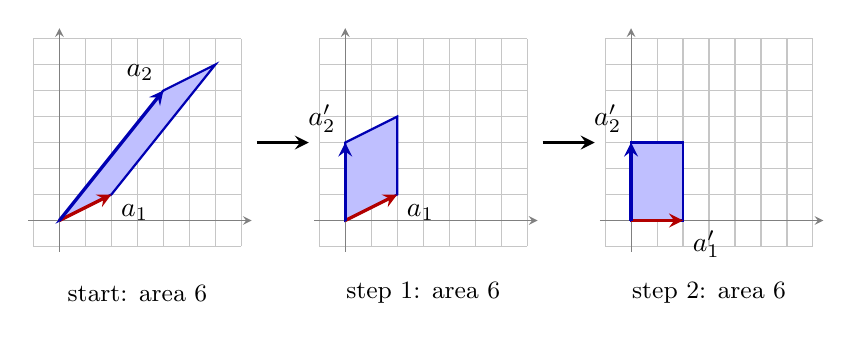
\begin{tikzpicture}[x=0.33cm,y=0.33cm,>=stealth]
  \draw[gray!45] (-1,-1) grid[step=1] (7,7);
  \draw[->,gray] (-1.2,0)--(7.4,0);
  \draw[->,gray] (0,-1.2)--(0,7.4);
  \fill[blue!25] (0,0)--(2,1)--(6,6)--(4,5)--cycle;
  \draw[thick,blue!70!black] (0,0)--(2,1)--(6,6)--(4,5)--cycle;
  \draw[->,very thick,red!70!black] (0,0)--(2,1);
  \draw[->,very thick,blue!70!black] (0,0)--(4,5);
  \node[below right] at (2,1) {$a_1$};
  \node[above left] at (4,5) {$a_2$};
  \node at (3,-2.8) {\small start: area 6};
  \draw[->,very thick] (7.6,3)--(9.6,3);
  \begin{scope}[shift={(11,0)}]
    \draw[gray!45] (-1,-1) grid[step=1] (7,7);
    \draw[->,gray] (-1.2,0)--(7.4,0);
    \draw[->,gray] (0,-1.2)--(0,7.4);
    \fill[blue!25] (0,0)--(2,1)--(2,4)--(0,3)--cycle;
    \draw[thick,blue!70!black] (0,0)--(2,1)--(2,4)--(0,3)--cycle;
    \draw[->,very thick,red!70!black] (0,0)--(2,1);
    \draw[->,very thick,blue!70!black] (0,0)--(0,3);
    \node[below right] at (2,1) {$a_1$};
    \node[above left] at (0,3) {$a_2'$};
    \node at (3,-2.8) {\small step 1: area 6};
    \draw[->,very thick] (7.6,3)--(9.6,3);
  \end{scope}
  \begin{scope}[shift={(22,0)}]
    \draw[gray!45] (-1,-1) grid[step=1] (7,7);
    \draw[->,gray] (-1.2,0)--(7.4,0);
    \draw[->,gray] (0,-1.2)--(0,7.4);
    \fill[blue!25] (0,0)--(2,0)--(2,3)--(0,3)--cycle;
    \draw[thick,blue!70!black] (0,0)--(2,0)--(2,3)--(0,3)--cycle;
    \draw[->,very thick,red!70!black] (0,0)--(2,0);
    \draw[->,very thick,blue!70!black] (0,0)--(0,3);
    \node[below right] at (2,0) {$a_1'$};
    \node[above left] at (0,3) {$a_2'$};
    \node at (3,-2.8) {\small step 2: area 6};
  \end{scope}
\end{tikzpicture}
\end{center}

\textbf{Figure.} The proof for $A=\begin{bmatrix}2&4\\1&5\end{bmatrix}$, with $\det A=10-4=6$. Left: the parallelogram spanned by $\bv{a}_1=(2,1)$ and $\bv{a}_2=(4,5)$. Step~1, the column replacement $C_2-2C_1$, replaces $\bv{a}_2$ by $\bv{a}_2'=(0,3)$: the top edge slides along the direction of $\bv{a}_1$ and the area does not change. Step~2, $C_1-\frac13C_2$, replaces $\bv{a}_1$ by $\bv{a}_1'=(2,0)$ and produces the $2\times3$ rectangle, of area $2\cdot3=6$.

\begin{exmp}{Area of a triangle from its vertices}{triangle}
A triangle with vertices $P_0,P_1,P_2$ is half of the parallelogram spanned by $\bv{u}=P_1-P_0$ and $\bv{v}=P_2-P_0$, translated to $P_0$. Hence
\[
\operatorname{area}=\tfrac12\left|\det[\bv{u}\ \ \bv{v}]\right|.
\]
For $P_0=(-1,0)$, $P_1=(3,1)$ and $P_2=(1,4)$ we get $\bv{u}=(4,1)$ and $\bv{v}=(2,4)$, so
\[
\operatorname{area}=\tfrac12\left|\begin{vmatrix}4&2\\1&4\end{vmatrix}\right|=\tfrac12|16-2|=7.
\]
Check by geometry: the triangle sits in the rectangle $[-1,3]\times[0,4]$ of area $16$, and the three corner triangles outside it have areas $\tfrac12\cdot4\cdot1=2$, $\ \tfrac12\cdot3\cdot2=3$ and $\tfrac12\cdot2\cdot4=4$, so the area is $16-9=7$. The same formula tests whether three points lie on a line, because that happens exactly when the area is $0$. For $(1,1)$, $(3,2)$, $(7,4)$ we get $\bv{u}=(2,1)$, $\bv{v}=(6,3)$ and $\det\begin{bmatrix}2&6\\1&3\end{bmatrix}=0$: the points are collinear.
\end{exmp}

\begin{exmp}{Volume of a parallelepiped}{volume}
Find the volume of the parallelepiped spanned by $(1,1,0)$, $(0,2,1)$ and $(1,0,3)$. Use them as the columns of
\[
A=\begin{bmatrix}1&0&1\\1&2&0\\0&1&3\end{bmatrix},\qquad
\det A=1\begin{vmatrix}2&0\\1&3\end{vmatrix}-0+1\begin{vmatrix}1&2\\0&1\end{vmatrix}=6+1=7,
\]
expanding along row $1$. The volume is $|\det A|=7$. If the third vector were $(1,3,1)$, the sum of the first two, the column operation $C_3-C_1-C_2$ would produce a zero column: the determinant is $0$ and the three edges lie in one plane, a flat parallelepiped of volume $0$.
\end{exmp}

\begin{kc}{Areas}{area}
(a)~Find the area of the parallelogram with vertices $(0,0)$, $(3,2)$, $(4,6)$ and $(1,4)$. (b)~Find the area of the triangle with vertices $(2,1)$, $(5,3)$ and $(3,6)$. (c)~Are the points $(1,1)$, $(3,2)$ and $(7,4)$ on one line?
\end{kc}

% ---------------------------------------------------------------------
\subsection*{Linear transformations and area}

Now let $T(\bv{x})=A\bv{x}$ be a linear transformation of the plane (or of space) and let $S$ be a region. We ask for the area of its image $T(S)=\{T(\bv{x}):\bv{x}\text{ in }S\}$.

\begin{thm}{Area and volume under a linear map}{scale}
Let $A$ be a $2\times2$ matrix and $T(\bv{x})=A\bv{x}$. If $S$ is a region in the plane that has an area, then
\[
\operatorname{area}\bigl(T(S)\bigr)=|\det A|\cdot\operatorname{area}(S).
\]
If $A$ is $3\times3$ and $S$ is a solid in space, then $\operatorname{vol}\bigl(T(S)\bigr)=|\det A|\cdot\operatorname{vol}(S)$.
\end{thm}

\begin{proof}
\emph{Parallelograms.} Let $S$ be the parallelogram $\{\bv{p}+s\bv{b}_1+t\bv{b}_2:0\leq s,t\leq1\}$ with corner $\bv{p}$, and let $B=[\bv{b}_1\ \bv{b}_2]$. By Theorem~\ref{thm:area}, $\operatorname{area}(S)=|\det B|$. Since $T$ is linear,
\[
T(\bv{p}+s\bv{b}_1+t\bv{b}_2)=A\bv{p}+s\,A\bv{b}_1+t\,A\bv{b}_2,
\]
so $T(S)$ is the parallelogram with corner $A\bv{p}$ spanned by $A\bv{b}_1$ and $A\bv{b}_2$. These are the columns of the product $AB$ (Section 2.1). A translation does not change area, so by Theorem~\ref{thm:area} and the product rule (Theorem~\ref{3.2-thm:product}),
\[
\operatorname{area}\bigl(T(S)\bigr)=|\det AB|=|\det A|\,|\det B|=|\det A|\cdot\operatorname{area}(S).
\]
The proof for parallelepipeds is the same with three columns.

\emph{General regions.} Fill $S$ with many tiny squares from a grid (cubes in space). Each square is a parallelogram, so its image has $|\det A|$ times its area, and the images of the squares fill $T(S)$. Adding up and letting the squares shrink multiplies the area of $S$ by $|\det A|$. This limit argument is how area is defined for general regions in calculus; we do not carry it out here.
\end{proof}

\begin{exmp}{The image of the unit disk}{disk}
Let $A=\begin{bmatrix}2&-1\\1&1\end{bmatrix}$, so $\det A=2+1=3$. The unit disk has area $\pi$, so its image under $T(\bv{x})=A\bv{x}$ has area $3\pi$. The image is a tilted ellipse: the disk is spanned by $\bv{e}_1$ and $\bv{e}_2$, which go to the columns $(2,1)$ and $(-1,1)$, and every other point is a combination of them. No formula for the area of a tilted ellipse was needed. For a matrix such as $\operatorname{diag}(a,b)$ the image is the ellipse with semi-axes $|a|$ and $|b|$, and the theorem gives $\pi|ab|$, the familiar area $\pi\times$ (one semi-axis) $\times$ (the other). In space the same argument shows that the ellipsoid with semi-axes $|a|,|b|,|c|$, the image of the unit ball under $\operatorname{diag}(a,b,c)$, has volume $\frac43\pi|abc|$.
\end{exmp}

\begin{center}
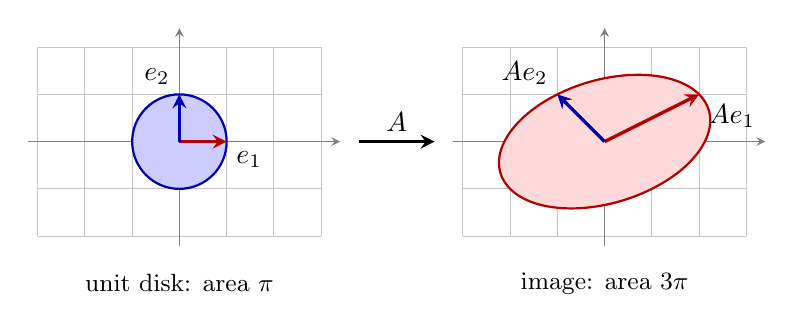
\begin{tikzpicture}[x=0.6cm,y=0.6cm,>=stealth]
  \draw[gray!45] (-3,-2) grid[step=1] (3,2);
  \draw[->,gray] (-3.2,0)--(3.4,0);
  \draw[->,gray] (0,-2.2)--(0,2.4);
  \draw[fill=blue!20,draw=blue!70!black,thick] (0,0) circle (1);
  \draw[->,very thick,red!70!black] (0,0)--(1,0);
  \draw[->,very thick,blue!70!black] (0,0)--(0,1);
  \node[below right] at (1,0) {$e_1$};
  \node[above left] at (0,1) {$e_2$};
  \node at (0,-3) {\small unit disk: area $\pi$};
  \draw[->,very thick] (3.8,0)--(5.4,0);
  \node[above] at (4.6,0) {$A$};
  \begin{scope}[shift={(9,0)}]
    \draw[gray!45] (-3,-2) grid[step=1] (3,2);
    \draw[->,gray] (-3.2,0)--(3.4,0);
    \draw[->,gray] (0,-2.2)--(0,2.4);
    \begin{scope}[cm={2,1,-1,1,(0,0)}]
      \draw[fill=red!15,draw=red!70!black,thick] (0,0) circle (1);
    \end{scope}
    \draw[->,very thick,red!70!black] (0,0)--(2,1);
    \draw[->,very thick,blue!70!black] (0,0)--(-1,1);
    \node[below right] at (2,1) {$Ae_1$};
    \node[above left] at (-1,1) {$Ae_2$};
    \node at (0,-3) {\small image: area $3\pi$};
  \end{scope}
\end{tikzpicture}
\end{center}

\textbf{Figure.} The matrix $A=\begin{bmatrix}2&-1\\1&1\end{bmatrix}$ carries the unit disk (area $\pi$) onto a tilted ellipse of area $|\det A|\,\pi=3\pi$. The arrows are the images $A\bv{e}_1=(2,1)$ and $A\bv{e}_2=(-1,1)$ of the two unit vectors.

\begin{exmp}{The image of a parallelogram}{parmap}
Let $S$ be the parallelogram with vertices $(1,1)$, $(3,2)$, $(4,5)$ and $(2,4)$, which is the corner $(1,1)$ plus the parallelogram spanned by $\bv{b}_1=(2,1)$ and $\bv{b}_2=(1,3)$. Then $\operatorname{area}(S)=\left|\det\begin{bmatrix}2&1\\1&3\end{bmatrix}\right|=5$. Let $A=\begin{bmatrix}2&-1\\1&3\end{bmatrix}$, so $\det A=7$ and the theorem predicts $\operatorname{area}(T(S))=35$. Apply $A$ to the four vertices:
\[
A\begin{bmatrix}1\\1\end{bmatrix}=\begin{bmatrix}1\\4\end{bmatrix},\quad
A\begin{bmatrix}3\\2\end{bmatrix}=\begin{bmatrix}4\\9\end{bmatrix},\quad
A\begin{bmatrix}4\\5\end{bmatrix}=\begin{bmatrix}3\\19\end{bmatrix},\quad
A\begin{bmatrix}2\\4\end{bmatrix}=\begin{bmatrix}0\\14\end{bmatrix}.
\]
The image is the parallelogram with corner $(1,4)$ and sides $(4,9)-(1,4)=(3,5)$ and $(0,14)-(1,4)=(-1,10)$, whose area is $\left|\det\begin{bmatrix}3&-1\\5&10\end{bmatrix}\right|=|30+5|=35$. \ $\checkmark$
\end{exmp}

\begin{exmp}{A shear, a rotation, a stretch and a projection}{fourmaps}
Let $S$ be the triangle with vertices $(0,0)$, $(3,0)$ and $(0,2)$, of area $\tfrac12\cdot3\cdot2=3$. Four maps from Section 1.9 act on it:
\[
\begin{array}{l|c|r|c|l}
\text{map}&\text{matrix}&\det A&\text{vertices of }T(S)&\text{area of }T(S)\\\hline
\text{shear}&\begin{bmatrix}1&1\\0&1\end{bmatrix}&1&(0,0),(3,0),(2,2)&3\\[8pt]
\text{rotation by }90^\circ&\begin{bmatrix}0&-1\\1&0\end{bmatrix}&1&(0,0),(0,3),(-2,0)&3\\[8pt]
\text{vertical stretch}&\begin{bmatrix}1&0\\0&3\end{bmatrix}&3&(0,0),(3,0),(0,6)&9\\[8pt]
\text{projection on the }x_1\text{-axis}&\begin{bmatrix}1&0\\0&0\end{bmatrix}&0&(0,0),(3,0),(0,0)&0
\end{array}
\]
In each case the area of the image is $|\det A|$ times $3$. The rotation by any angle $\theta$ has $\det\begin{bmatrix}\cos\theta&-\sin\theta\\\sin\theta&\cos\theta\end{bmatrix}=\cos^2\theta+\sin^2\theta=1$: rotations keep every area. The projection has $\det A=0$ and flattens the triangle onto a segment, which has area $0$.
\end{exmp}

\begin{center}
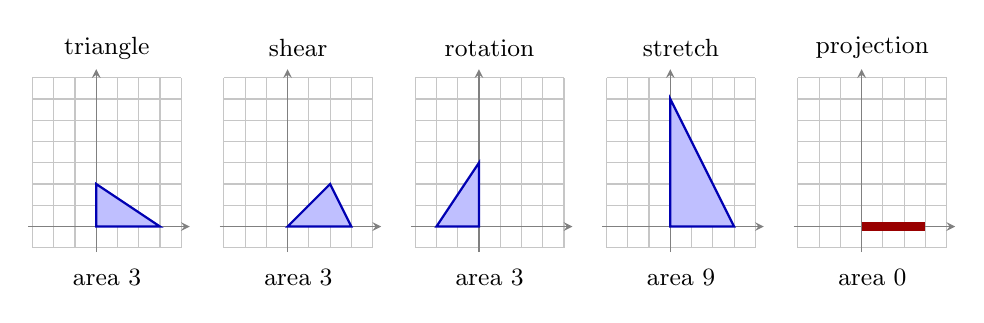
\begin{tikzpicture}[x=0.27cm,y=0.27cm,>=stealth]
  \foreach \cx in {0,9,18,27,36}{
    \begin{scope}[shift={(\cx,0)}]
      \draw[gray!45] (-3,-1) grid[step=1] (4,7);
      \draw[->,gray] (-3.2,0)--(4.4,0);
      \draw[->,gray] (0,-1.2)--(0,7.4);
    \end{scope}}
  \begin{scope}[shift={(0,0)}]
    \draw[thick,blue!70!black,fill=blue!25] (0,0)--(3,0)--(0,2)--cycle;
    \node at (0.5,8.4) {\small triangle};
    \node at (0.5,-2.4) {\small area 3};
  \end{scope}
  \begin{scope}[shift={(9,0)}]
    \draw[thick,blue!70!black,fill=blue!25] (0,0)--(3,0)--(2,2)--cycle;
    \node at (0.5,8.4) {\small shear};
    \node at (0.5,-2.4) {\small area 3};
  \end{scope}
  \begin{scope}[shift={(18,0)}]
    \draw[thick,blue!70!black,fill=blue!25] (0,0)--(0,3)--(-2,0)--cycle;
    \node at (0.5,8.4) {\small rotation};
    \node at (0.5,-2.4) {\small area 3};
  \end{scope}
  \begin{scope}[shift={(27,0)}]
    \draw[thick,blue!70!black,fill=blue!25] (0,0)--(3,0)--(0,6)--cycle;
    \node at (0.5,8.4) {\small stretch};
    \node at (0.5,-2.4) {\small area 9};
  \end{scope}
  \begin{scope}[shift={(36,0)}]
    \draw[line width=3pt,red!60!black] (0,0)--(3,0);
    \node at (0.5,8.4) {\small projection};
    \node at (0.5,-2.4) {\small area 0};
  \end{scope}
\end{tikzpicture}
\end{center}

\textbf{Figure.} The triangle with vertices $(0,0)$, $(3,0)$, $(0,2)$ and its images under the four maps of Example~\ref{ex:fourmaps}. The shear and the rotation keep the area, the stretch multiplies it by $3$, and the projection squeezes the triangle onto a segment.

\begin{think}{What does the sign of $\det A$ record?}{sign}
Let $S$ be the triangle of Example~\ref{ex:fourmaps} with vertices $O=(0,0)$, $P=(3,0)$ and $Q=(0,2)$; going $O\to P\to Q$ turns counterclockwise. (a)~Find the images of $O,P,Q$ under the interchange matrix $\begin{bmatrix}0&1\\1&0\end{bmatrix}$, which has determinant $-1$. In which direction does the image triangle turn? (b)~Which of the shear, rotation and stretch keep the direction of the turn, and what are the signs of their determinants? (c)~The stretch $\begin{bmatrix}-2&0\\0&1\end{bmatrix}$ has $\det=-2$. Find the image of $S$, its area, and the direction of its turn. (d)~Summarize what $\det A>0$, $\det A<0$ and $\det A=0$ each say about the picture.
\end{think}

\begin{think}{Why $|\det A|$ and not $\det A$?}{abs}
(a)~The interchange matrix above has $\det=-1$ and sends the triangle of area $3$ to a triangle of area $3$. What would ``area $\times\det A$'' give, and is that possible for an area? (b)~Both $\det A$ and $|\det A|$ satisfy the product rule. Why can the product rule alone not decide which one is the area scale factor? (c)~What information does $\det A$ carry that $|\det A|$ throws away?
\end{think}

\begin{think}{Composition and the product of scale factors}{compose}
Let $A=\begin{bmatrix}1&1\\0&1\end{bmatrix}$ (a shear) and $B=\begin{bmatrix}1&0\\0&3\end{bmatrix}$ (a stretch). (a)~Compute $AB$ and $BA$. Are they equal? Find the images of the unit square under the maps with matrices $AB$ and $BA$. (b)~By what number does each of $A$ and $B$ multiply areas? Compute $|\det AB|$ and $|\det BA|$. (c)~Use Theorem~\ref{3.2-thm:product} and Theorem~\ref{thm:scale} to explain why the composite ``first $A$, then $B$'' multiplies every area by $|\det B|\,|\det A|$, and why the order changes the image but not the factor. (d)~One map multiplies areas by $\tfrac12$ and a second by $8$. What is the factor for their composite, and for the inverse of the composite?
\end{think}

\begin{kc}{Scale factors}{scale}
(a)~$A=\begin{bmatrix}3&1\\2&4\end{bmatrix}$ maps a region of area $7$ to a region of what area? (b)~A $3\times3$ matrix with $\det=-2$ maps a solid of volume $5$ to a solid of what volume? (c)~The matrix $\begin{bmatrix}5&0\\0&2\end{bmatrix}$ maps the unit disk to an ellipse. What is its area, and does it agree with $\pi ab$? (d)~A region of area $4$ is mapped by $A=\begin{bmatrix}1&2\\h&3\end{bmatrix}$ to a region of area $10$. Find $h$ (there are two values).
\end{kc}

\subsection*{Summary}
\begin{itemize}
  \item \textbf{Cramer's Rule.} If $\det A\neq0$, the solution of $A\bv{x}=\bv{b}$ is $x_i=\det A_i(\bv{b})/\det A$, where $A_i(\bv{b})$ is $A$ with column $i$ replaced by $\bv{b}$. The proof is $A\,I_i(\bv{x})=A_i(\bv{b})$ plus the product rule. \textbf{Always build $A_i(\bv{b})$ from the original $A$.}
  \item If $\det A=0$ the rule does not apply: a nonzero $\det A_i(\bv{b})$ proves there is no solution, while all $\det A_i(\bv{b})=0$ proves nothing.
  \item \textbf{Cost.} Cramer's Rule needs $n+1$ determinants. It is useful for $2\times2$ and $3\times3$ systems and for formulas with parameters, and it is a poor way to solve large systems: row reduction of $[A\ \ \bv{b}]$ is about $n+1$ times cheaper even when every determinant is computed by elimination.
  \item \textbf{Adjugate.} $\operatorname{adj}A$ is the \textbf{transpose} of the cofactor matrix, and $A^{-1}=\frac1{\det A}\operatorname{adj}A$. For $2\times2$ matrices this is the formula of Section 2.2.
  \item \textbf{Geometry.} The parallelogram spanned by the columns of a $2\times2$ matrix has area $|\det A|$, the parallelepiped spanned by the columns of a $3\times3$ matrix has volume $|\det A|$, and a triangle with vertices $P_0,P_1,P_2$ has area $\tfrac12|\det[P_1-P_0\ \ P_2-P_0]|$.
  \item \textbf{Linear maps.} $T(\bv{x})=A\bv{x}$ multiplies the area (volume) of \emph{every} region by $|\det A|$; the factors of a composite multiply; $\det A=0$ flattens. The sign of $\det A$ records whether orientation is kept or reversed.
\end{itemize}

\subsection*{Questions to think about before the next section}
\begin{enumerate}
  \item By Cramer's Rule, $x_i=\det A_i(\bv{b})/\det A$. What happens to the solution when $\det A$ is very close to $0$ and the numerator is not? Compare with the nearly singular matrix of Example~\ref{2.3-ex:nearly}.
  \item The formula $A^{-1}=\frac1{\det A}\operatorname{adj}A$ shows that a matrix with integer entries and $\det A=\pm1$ has an inverse with integer entries. Why? Is the converse true?
  \item The image of the unit disk under $\bv{x}\mapsto A\bv{x}$ is an ellipse of area $\pi|\det A|$. When is that ellipse a circle? Experiment with a rotation, a stretch and a shear.
\end{enumerate}

\subsection*{Answers and discussion}
\begin{description}[leftmargin=0pt,itemsep=5pt]
  \item[Knowledge Check \ref{kc:replace}.] (a)~$A_2(\bv{b})=\begin{bmatrix}1&1&7\\2&0&8\\3&2&10\end{bmatrix}$ and $A_3(\bv{b})=\begin{bmatrix}1&4&1\\2&5&0\\3&6&2\end{bmatrix}$: column $2$ (respectively column $3$) of $A$ is replaced by $\bv{b}$, and the other columns are those of $A$. (b)~The denominator is $\det A=-3$ for all three unknowns. (c)~$A_1(\bv{b})=\begin{bmatrix}1&4&7\\0&5&8\\2&6&10\end{bmatrix}$. Expanding down column $1$ (entries $1,0,2$): $\det A_1(\bv{b})=1(50-48)+2(32-35)=2-6=-4$, so $x_1=\frac{-4}{-3}=\frac43$. (For completeness, $\det A_2(\bv{b})=16$ and $\det A_3(\bv{b})=-9$, so $\bv{x}=(\tfrac43,-\tfrac{16}3,3)$; check the third equation: $4-32+30=2$.)
  \item[Knowledge Check \ref{kc:adj}.] (a)~The cofactors are $C_{11}=2$, $C_{12}=-4$, $C_{21}=-1$, $C_{22}=3$, so $\operatorname{adj}A=\begin{bmatrix}2&-1\\-4&3\end{bmatrix}$ and $\det A=6-4=2$. Hence $A^{-1}=\frac12\begin{bmatrix}2&-1\\-4&3\end{bmatrix}$, which is the $2\times2$ formula. (b)~The cofactors are $C_{11}=1,\ C_{12}=0,\ C_{13}=0,\ C_{21}=-1,\ C_{22}=1,\ C_{23}=0,\ C_{31}=1,\ C_{32}=-1,\ C_{33}=1$, so the cofactor matrix is $\begin{bmatrix}1&0&0\\-1&1&0\\1&-1&1\end{bmatrix}$ and $\operatorname{adj}A=\begin{bmatrix}1&-1&1\\0&1&-1\\0&0&1\end{bmatrix}$. Since $\det A=1$, $A^{-1}=\operatorname{adj}A$. (c)~$A$ times the cofactor matrix has first row $(1\cdot1+1\cdot(-1),\ 1,\ 0)=(0,1,0)$, not $(1,0,0)$, so it is not the inverse. The slip is forgetting the transpose. (Also, the inverse of an upper triangular matrix is upper triangular here, which the lower triangular matrix cannot be.)
  \item[Knowledge Check \ref{kc:area}.] (a)~The parallelogram is spanned by $(3,2)$ and $(1,4)$, so the area is $\left|\det\begin{bmatrix}3&1\\2&4\end{bmatrix}\right|=|12-2|=10$. (b)~$\bv{u}=(3,2)$ and $\bv{v}=(1,5)$, so the area is $\tfrac12|15-2|=\tfrac{13}2$. (c)~$\bv{u}=(2,1)$ and $\bv{v}=(6,3)$ give $\det=6-6=0$, so the points are collinear (indeed $\bv{v}=3\bv{u}$).
  \item[Knowledge Check \ref{kc:scale}.] (a)~$\det A=12-2=10$, so the area is $70$. (b)~$|{-2}|\cdot5=10$. (c)~$\det=10$, so the area is $10\pi$; the image is the ellipse with semi-axes $5$ and $2$, and $\pi ab=10\pi$. (d)~$\det A=3-2h$, and the factor is $\frac{10}4=\frac52$, so $|3-2h|=\frac52$: either $3-2h=\frac52$, $h=\frac14$, or $3-2h=-\frac52$, $h=\frac{11}4$.
  \item[Pause and think \ref{think:why}.] (a)~$I_1(\bv{x})=\begin{bmatrix}x_1&0\\x_2&1\end{bmatrix}$ and $AI_1(\bv{x})=\begin{bmatrix}ax_1+bx_2&b\\cx_1+dx_2&d\end{bmatrix}=\begin{bmatrix}b_1&b\\b_2&d\end{bmatrix}$, which is $A_1(\bv{b})$ for $\bv{b}=A\bv{x}$. Similarly $I_2(\bv{x})=\begin{bmatrix}1&x_1\\0&x_2\end{bmatrix}$ and $AI_2(\bv{x})=\begin{bmatrix}a&b_1\\c&b_2\end{bmatrix}=A_2(\bv{b})$. (b)~Column $j$ of a product $AM$ is $A$ times column $j$ of $M$. For $j\neq i$ column $j$ of $I_i(\bv{x})$ is $\bv{e}_j$, and $A\bv{e}_j$ is column $j$ of $A$; column $i$ is $A\bv{x}=\bv{b}$ because $\bv{x}$ is a solution. (c)~$I_3(\bv{x})=\begin{bmatrix}1&0&x_1\\0&1&x_2\\0&0&x_3\end{bmatrix}$ is upper triangular, so its determinant is the product of the diagonal entries, $x_3$ (Theorem~\ref{3.1-thm:triangular}). $I_2(\bv{x})=\begin{bmatrix}1&x_1&0\\0&x_2&0\\0&x_3&1\end{bmatrix}$ is not triangular, but expansion along row $2$ gives $x_2$; in general this is the expansion used in the proof.
  \item[Pause and think \ref{think:hyp}.] (a)~Two steps need $\det A\neq0$: the existence of the solution $\bv{x}$ used at the start (Theorem~\ref{2.2-thm:solve} needs $A$ invertible) and the final division by $\det A$. (b)~$\det A=4-4=0$. For $\bv{b}=(3,6)$: $\det A_1(\bv{b})=\begin{vmatrix}3&2\\6&4\end{vmatrix}=0$ and $\det A_2(\bv{b})=\begin{vmatrix}1&3\\2&6\end{vmatrix}=0$; the system $x_1+2x_2=3$, $2x_1+4x_2=6$ has infinitely many solutions. For $\bv{b}=(3,5)$: $\det A_1(\bv{b})=12-10=2$ and $\det A_2(\bv{b})=5-6=-1$; the system $x_1+2x_2=3$, $2x_1+4x_2=5$ has no solution. (c)~Then $0\cdot x_i=\det A_i(\bv{b})$, so every $\det A_i(\bv{b})=0$. Contrapositive: if some $\det A_i(\bv{b})\neq0$ there is no solution. Conversely, all numerators equal to $0$ is consistent with infinitely many solutions (as for $\bv{b}=(3,6)$) but does not prove that a solution exists, and it does not single one out.
  \item[Pause and think \ref{think:cost}.] (a)~$n+1$. (b)~At least $11\cdot10!=39{,}916{,}800$ multiplications, about eleven times the cost of one determinant. (c)~$101\cdot\tfrac23\cdot100^3\approx6.7\times10^7$ operations for Cramer's Rule, against $\tfrac23\cdot100^3\approx6.7\times10^5$ for one row reduction of $[A\ \ \bv{b}]$. (d)~By a factor of about $n+1=101$; in addition, the row reduction that computes $\det A$ has already done the work needed to solve the system. (e)~Two reasons: the rule gives a \emph{formula} showing how each unknown depends on $\bv{b}$ (it is a linear function of $\bv{b}$) and on parameters, as in Example~\ref{ex:param}; and it is the key to the adjugate formula for the inverse and to theoretical statements about solutions. For $2\times2$ and $3\times3$ systems by hand it is also perfectly practical.
  \item[Pause and think \ref{think:sign}.] (a)~$O\mapsto(0,0)$, $P\mapsto(0,3)$, $Q\mapsto(2,0)$. Going $O\to P'\to Q'$ means up the $x_2$-axis and then to $(2,0)$: the turn is clockwise. (b)~The shear (image $(0,0),(3,0),(2,2)$) and the rotation (image $(0,0),(0,3),(-2,0)$) and the stretch (image $(0,0),(3,0),(0,6)$) all still turn counterclockwise; their determinants $1$, $1$, $3$ are positive. (c)~$P\mapsto(-6,0)$, $Q\mapsto(0,2)$, so the image has vertices $(0,0),(-6,0),(0,2)$, area $\tfrac12\cdot6\cdot2=6=2\cdot3$, and $O\to P'\to Q'$ turns clockwise. The matrix reflects in the $x_2$-axis and stretches by $2$. (d)~$\det A>0$: the map keeps orientation; $\det A<0$: it reverses orientation (a reflection is involved); $\det A=0$: the plane is flattened onto a line or a point and nothing is left to orient.
  \item[Pause and think \ref{think:abs}.] (a)~``Area $\times\det A$'' would give $3\cdot(-1)=-3$, and an area cannot be negative. (b)~Both satisfy $f(AB)=f(A)f(B)$. The product rule is a statement about multiplication and cannot tell the two apart; what decides is that areas are nonnegative and that the unit square, of area $1$, goes to the parallelogram of area $|\det A|$ (Theorem~\ref{thm:area}). (c)~The sign: whether the map preserves or reverses orientation. It is lost in $|\det A|$, and it is useful whenever the direction of travel around a region matters.
  \item[Pause and think \ref{think:compose}.] (a)~$AB=\begin{bmatrix}1&3\\0&3\end{bmatrix}$ and $BA=\begin{bmatrix}1&1\\0&3\end{bmatrix}$; they are not equal. The unit square goes under $AB$ to the parallelogram with vertices $(0,0),(1,0),(4,3),(3,3)$ and under $BA$ to $(0,0),(1,0),(2,3),(1,3)$: different shapes. (b)~$A$ has $|\det A|=1$ and $B$ has $|\det B|=3$; $|\det AB|=3=|\det BA|$, and both parallelograms have area $3$. (c)~By Theorem~\ref{thm:scale} the first map multiplies every area by $|\det A|$, and applying it to the image region, the second map multiplies that area by $|\det B|$: the composite multiplies by $|\det B||\det A|$. The composite has matrix $BA$ (the matrix of a composite is the product of the matrices, Section 2.1), and Theorem~\ref{3.2-thm:product} gives $|\det BA|=|\det B||\det A|$, the same number. The numbers $|\det A|$ and $|\det B|$ commute, although the matrices do not, so the order changes the image but not its area. (d)~The composite multiplies areas by $\tfrac12\cdot8=4$ and its inverse by $\tfrac14$.
  \item[Before the next section.] (1)~If $\det A$ is close to $0$ while the numerator is not, then $x_i$ is huge, and a tiny change in $\bv{b}$ (hence in the numerator) can change $x_i$ greatly. This is the large inverse of Example~\ref{2.3-ex:nearly}: there $\det A=0.0001$. (2)~Each entry of $\operatorname{adj}A$ is a cofactor, an integer when $A$ has integer entries, and dividing by $\det A=\pm1$ keeps it an integer. The converse is also true (Homework) and uses the product rule: $\det A\det A^{-1}=1$ with both determinants integers. (3)~The image is a circle exactly when $A$ maps the unit circle to a circle: a rotation does (its determinant is $\pm1$ for rotations and reflections), and so does a multiple $rI$ of the identity; a stretch with different factors or a shear turns the circle into a genuine ellipse. The area $\pi|\det A|$ alone does not tell the shape.
\end{description}

\end{document}
